\input{includeFile}

\long\def\omitit #1{}

\begin{document}



\MYTITLE{Lab 3:\\ Translation with Python3}
\MYHEADERS{}{\color{red} Due: 23$^{rd}$ Sept\color{black}}{Handed out: 16$^{th}$ Sept. 2019}
% Due: 9$^{th}$ Sept
\flushleft

\begin{figure}[ht!]
	\begin{center}
	 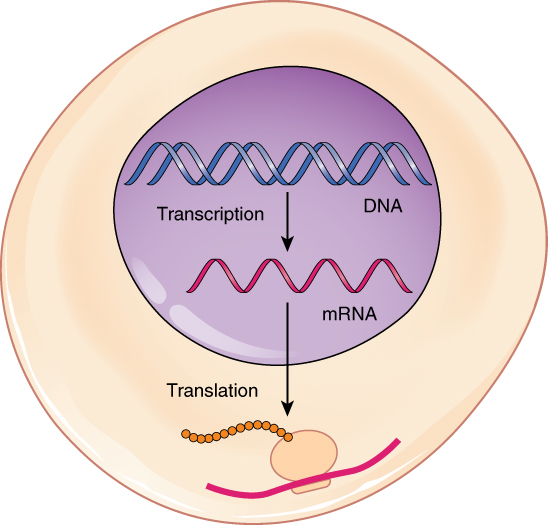
\includegraphics[scale=.5]{graphics/dogma.jpg}
	\end{center}
	\caption{The central dogma of biology in a nutshell (i.e., DNA $\to$ RNA $\to$ Protein.)}
	\label{fig:dogma}
\end{figure}


%\MYTITLE{Lab 3: \\ \color{red}Save this lab assignment to: {\tt labs/lab3}\color{black}}
%\MYHEADERS{Introduction to Bioinformatics}{Due: 20 Sept.}{Handed out on: 13 Sept. 2017}

%In this lab assignment you are invited to review your understanding of  biological concepts behind transcription, translation and mutation processes and to continue building on your Python programming skills.



\subsubsection*{GitHub starter link}
\begin{center}
\color{red} \url{https://classroom.github.com/a/zn0wOF2R} \color{black}
\end{center}



To use this link, please follow the steps below.
\begin{itemize}
	\item Click on the link and accept the assignment.
	\item Once the importing task has completed, click on the created assignment link which will take you to your newly created GitHub repository for this lab.
	\item Clone this repository (bearing your name) and work on the practical locally.
	\item As you are working on your practical, you are to commit and push regularly. You can use the following commands to add a single file, you must be in the directory where the file is located (or add the path to the file in the command):
		\begin{itemize}
		\item {\tt git add -A}
		\item {\tt git commit -m ``Your notes about commit here''}
		\item {\tt git push}
	\end{itemize}

	Alternatively, you can use the following commands to add multiple files from your repository:
	\begin{itemize}
		\item {\tt git commit <}\emph{nameOfFile}\tt{> -m ``Your notes about commit here''}
		\item {\tt git push}
	\end{itemize}
\end{itemize}
%%%

Be sure to read the {\tt README.md} file in the GitHub Classroom repository for instructions on how to complete your first assignment.


\begin{figure}[ht!]
	\begin{center}
	 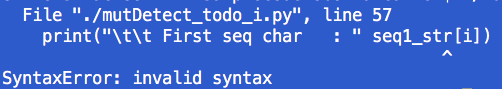
\includegraphics[scale=.5]{graphics/bugs.png}
	\end{center}
	\caption{Finding bugs in code is a normal part of programming.}
	\label{fig:bugs}
\end{figure}

\subsection*{Objectives}

To strengthen the understanding of the transcription, translation and mutation. To learn to debug Python3 code that performs a basic analysis of sequences using transcription and translation.

\vspace*{-.1in}
\subsection*{Reading Assignment}
\vspace*{-.1in}
In addition to following the specified sections of the Python tutorial outlined below, please read Chapter 3 in the ``ThinkPython'' book. You should also review class slides and videos on the topics of transcription, translation and mutation. 


\section*{Analysis Program}

The program that you have been given in the {\color{red} \tt src/mutDetect\_todo\_i.py \color{black}} is supposed to compare sequences and to perform basic translations of two user-entered sequences. It is then supposed to compare the protein sequences of the two DNA sequences to find changes in product. Unfortunately, this code was written hastily and, as a result, contains TWELVE (12) basic coding bugs (i.e., typographical errors) that prevent the code from working properly. \textbf{Your task is to complete the code by fixing the errors to allow it to run and to display the output shown below.}



Your output should look like the following.

\begin{verbatim}
bioinformaticsNumberOneFan$ ./mutDetect.py s

	 Welcome to mutDetect!
	 A program to compare DNA, make protein and compare protein sequences.
 __Getting a sequence__
	Enter a sequence :atgatgatggcc
 __Getting a sequence__
	Enter a sequence :atgatgatgggg
	 + Length of first sequence  : 12
	 + Length of second sequence : 12

 __Comparing sequences__
	 + Bases not the same at pos:  10
		 First seq char   :  c
		 Second  seq char :  g
	 + Bases not the same at pos:  11
		 First seq char   :  c
		 Second  seq char :  g
	 + Sequences are same length:  True

 __Translation__
	 + Original DNA       : atgatgatggcc , length is : 12
	 + PROTEIN from RNA   : MMMA
	 + protein1 sequence  : MMMA

 __Translation__
	 + Original DNA       : atgatgatgggg , length is : 12
	 + PROTEIN from RNA   : MMMG
	 + protein2 sequence  : MMMG

 __Comparing sequences__
	 + Bases not the same at pos:  3
		 First seq char   :  A
		 Second  seq char :  G

\end{verbatim}




\vspace*{-.2in}
\subsection*{Required Deliverables}
\vspace*{-.1in}

\begin{itemize}
	\item Your completed activity should be saved as {\color{red} \tt src/mutDetect\_todo\_i.py \color{black}} in the repository that you will push to GitHub.


    \item Write a reflection of about 100 words to describe your approach to finding the errors of the code. Record your reflection in the markdown document; {\tt \color{red} writing/reflections.md\color{black}}.	
	\end{itemize}

\noindent Please see the instructor if you have questions about the assignment submission.

\end{document}

%%%% junk bin %%%%%
%%%% junk bin %%%%%
%%%% junk bin %%%%%
%%%% junk bin %%%%%
%%%% junk bin %%%%%
%%%% junk bin %%%%%
%%%% junk bin %%%%%

%%%%%%%%%%%
% working code

#!/usr/bin/env python3

# Originally written by: Oliver Bonham-Carter
# email:
# Date: 13 Sept 2019
# Comment: A DNA translator and mutation detector.

# Library installation notes:
#
# Commands to install biopython
# python3 -m pip install biopython # global install
# python3 -m pip install biopython –user # local install

############################################################################
# TODO: In the other file, there are twelve bugs to fix. Did you find them?!
############################################################################


DATE = "16 Sept 2019"
VERSION = "i"
AUTHOR = " myName"
AUTHORMAIL = "@allegheny.edu"

def help():
        h_str = "   "+DATE+" | version: "+VERSION+" |"+AUTHOR+" | "+AUTHORMAIL
        print("  "+len(h_str) * "-")
        print(h_str)
        print("  "+len(h_str) * "-")
        print("\n\tThe blank-blank program to do something cool.")
        #print("""\n\tLibrary installation notes:""")
        print("\t+ \U0001f600  USAGE: python3 mutDetect.py <any key to launch>")

######################################################
#end of help()


def getSeq():
    """ Function to get a sequence (a string) from the user"""
    print(" __Getting a sequence__")

    prmpt = "\tEnter a sequence :"
    seq_str = input(prmpt)
    return seq_str.lower()

######################################################
# end of getSeq()


def compareSequences(seq1_str, seq2_str):
    """ Compares the sequences base by base"""
    print("\n __Comparing sequences__")

    for i in range(len(seq1_str)):
        # check to see whether the bases are the same going through the sequences
        try:
            if seq1_str[i] != seq2_str[i]: # are bases _not_ the same at the same position?
                print("\t + Bases not the same at pos: ",i)
                print("\t\t First seq char   : ", seq1_str[i])
                print("\t\t Second  seq char : ", seq2_str[i])
        except IndexError:
            #print(" \t Sequences are uneven length!")
            pass
# end of compareSequences()

def getSeqLength(seq_str):
    """ Function to return the length of a sequence"""
    l_int = len(seq_str)
    if l_int % 3 != 0: # can we read triplets, groups of three?
        print("\t Warning! Sequence length cannot be divided into groups of triplets!")
    return l_int
######################################################
#end of getSeqLength()

def compareSeqLength(seq1_str, seq2_str):
    """Function to check the lengths of the sequences to make sure that they are the same length. This is necessary for making comparisons."""
    if len(seq1_str) != len(seq2_str):
        return False
    else:
        return True
######################################################
#end of compareSeqLength()

def translate(dna_str):
    """ Function to translate the DNA. Create a protein sequence from the DNA."""

    sequence = Seq(dna_str)
    #make some variables to hold strings of the translated code
    # give me RNA from the DNA
    RNAfromDNA_str = Seq.transcribe(sequence) #transcription step: converting dna to rna
    # give me DNA from the RNA
    DNAfromRNA_str = Seq.back_transcribe(sequence)
    # give me the protein from the dna
    PROTfromRNA_str = Seq.translate(RNAfromDNA_str)

    # print the output of the string variables
    print("\n __Translation__")

    print("\t + Original DNA       :", dna_str, ", length is :", len(dna_str))
    # print("\t + RNA from DNA     :", RNAfromDNA_str)
    # print("\t + DNA from RNA     :", DNAfromRNA_str)
    print("\t + PROTEIN from RNA   :",PROTfromRNA_str)

    return PROTfromRNA_str
######################################################
#end of translate()



def begin(task_str):
    """Driver function of program"""
    print("\n\t Welcome to mutDetect!\n\t A program to compare DNA, make protein and compare protein sequences.")
# get first DNA sequence
    seq1_str = getSeq()
# get second DNA sequence
    seq2_str = getSeq()

    print("\t + Length of first sequence  :", getSeqLength(seq1_str))
    print("\t + Length of second sequence :", getSeqLength(seq2_str))

# compare the sequences
    compareSequences(seq1_str, seq2_str)
    print("\t + Sequences are same length: ",compareSeqLength(seq1_str, seq2_str))

    prot1_seq = translate(seq1_str)
    #print(type(prot1_seq))
    protein1_str = str(prot1_seq)
    print("\t + protein1 sequence  :",protein1_str)

    prot2_seq = translate(seq2_str)
    #print(type(prot2_seq))
    protein2_str = str(prot2_seq)
    print("\t + protein2 sequence  :",protein2_str)

    compareSequences(protein1_str, protein2_str)

######################################################
#end of begin()



import os, sys
#import math
# list other libraries below

# load my biopython library
from Bio.Seq import Seq


if __name__ == '__main__':

        if len(sys.argv) == 2: # one parameter at command line
        # note: the number of command line parameters is n + 1
                begin(sys.argv[1])
        else:
                help() # If no command-line parameter entered, then run the help() function
                sys.exit()

% end of working code
%%%%%%%%%%%%%%%%
%%%%%%%%%%%%%%%%
%%%%%%%%%%%%%%%%
%%%%%%%%%%%%%%%%
%%%%%%%%%%%%%%%%



%%%%%%%%%%%
% buggy code

#!/usr/bin/env python3

# Originally written by: Oliver Bonham-Carter
# email:
# Date: 13 Sept 2019
# Comment: A DNA translator and mutation detector.

# Library installation notes:
#
# Commands to install biopython
# python3 -m pip install biopython # global install
# python3 -m pip install biopython –user # local install

############################################################################
# TODO: There are twelve EMBARRISING silly bugs to fix. Can you find them?!
############################################################################

DATE = "16 Sept 2019"
VERSION = "i"
AUTHOR = " myName"
AUTHORMAIL = "@allegheny.edu"

def help():
        h_str = "   "+DATE+" | version: "+VERSION+" |"+AUTHOR+" | "+AUTHORMAIL
        print("  "+len(h_str) * "-")
        print(h_str)
        print("  "+len(h_str) * "-")
        print("\n\tThe blank-blank program to do something cool.")
        #print("""\n\tLibrary installation notes:""")
        print("\t+ \U0001f600  USAGE: python3 mutDetect.py <any key to launch>")

######################################################
#end of help()


def getSeq():
    """ Function to get a sequence (a string) from the user"""
    print(" __Getting a sequence__")

    prmpt = "\tEnter a sequence :"
    seq_str = int(input(prmpt))
    return seq_str.lower()

######################################################
# end of getSeq()


def compareSequences(seq1_str, seq2_str):
    """ Compares the sequences base by base"""
    print("\n __Comparing sequences__")

    for i in range(len(seq1_str)):
        # check to see whether the bases are the same going through the sequences
        try:
            if seq1_str[i] == seq2_str[i]: # are bases _not_ the same at the same position?
                print("\t + Bases not the same at pos: ",i)
                print("\t\t First seq char   : " seq1_str[i])
                print("\t\t Second  seq char : ", seq2_str[i])
        except IndexError:
            #print(" \t Sequences are uneven length!")
            pass
# end of compareSequences()

def getSeqLength(seq_str):
    """ Function to return the length of a sequence"""
    l_int = len(seq_str)
    if l_int % 2 = 0: # can we read triplets, groups of three?
        print("\t Warning! Sequence length cannot be divided into groups of triplets!")
    return l_int
######################################################
#end of getSeqLength()

def compareSeqLength(seq1_str, seq2_str):
    """Function to check the lengths of the sequences to make sure that they are the same length. This is necessary for making comparisons."""
    if len(seq1_str) = len(seq2_str):
        return True
    else:
        return True
######################################################
#end of compareSeqLength()

def translate(dna_str):
    """ Function to translate the DNA. Create a protein sequence from the DNA."""

    sequence = Seq(dna_str)
    #make some variables to hold strings of the translated code
    # give me RNA from the DNA
    RNAfromDNA_str = Seq.transcribe(sequence) #transcription step: converting dna to rna
    # give me DNA from the RNA
    DNAfromRNA_str = Seq.back_transcribe(sequence)
    # give me the protein from the dna
    PROTfromRNA_str = Seq.translate(RNAfromDNA_str)

    # print the output of the string variables
    print("\n __Translation__")

    print("\t + Original DNA       :", dna_str ", length is :", len(dna_str))
    # print("\t + RNA from DNA     :", RNAfromDNA_str)
    # print("\t + DNA from RNA     :", DNAfromRNA_str)
    print("\t + PROTEIN from RNA   :",PROTfromRNA_str)

    return PROTfromRNA_str
######################################################
#end of translate()



def begin(task_str):
    """Driver function of program"""
    print("\n\t Welcome to mutDetect!\n\t A program to compare DNA, make protein and compare protein sequences.)
# get first DNA sequence
    seq1_str = getSeq()
# get second DNA sequence
    seq2_str = getSeq()

    print("\t + Length of first sequence  :", getSeqLength(seq2_str))
    print("\t + Length of second sequence :", getSeqLength(seq2_str))

# compare the sequences
    compareSeQuences(seq1_str, seq2_str)
    print("\t + Sequences are same length: ",compareSeqLength(seq1_str, seq2_str))

    prot1_seq = Translate(seq1_str)
    #print(type(prot1_seq))
    protein1_str = str(prot1_seq)
    print("\t + protein1 sequence  :",protein1_str)

    prot2_seq = translate(seq2_tsr)
    #print(type(prot2_seq))
    protein2_str = str(prot2_seq)
    print("\t + protein2 sequence  :",protein2_str)

    compareSequences(protein1_str, protein2_str)

######################################################
#end of begin()



import os, sys
#import math
# list other libraries below

# load my biopython library
from Bio.Seq import Seq


if __name__ == '__main__':

        if len(sys.argv) == 2: # one parameter at command line
        # note: the number of command line parameters is n + 1
                begin(sys.argv[1])
        else:
                help() # If no command-line parameter entered, then run the help() function
                sys.exit()


% end of buggy code
%%%%%%%%%%%%%%%%


